\chapter{Scalaz} % Main chapter title

\label{Chapter1} % Change X to a consecutive number; for referencing this chapter elsewhere, use \ref{ChapterX}

Scalaz è una libreria open source per la programmazione funzionale, che mette a disposizione un grande numero di strutture dati puramente funzionali create per integrare quelle della Scala Standard Library. In Scalaz sono presenti diversi nuovi elementi, definiti principalmente sotto forma di type class, ma anche delle estensioni per le strutture dati standard.

Scalaz rappresenta un progetto molto ampio, tanto che la prima release risale al 2010 e l'ultima a pochi giorni fa e che si sono sviluppati diversi progetti a partire da esso (come ad esempio Scalaz IO, poi trasformatosi nello standalone ZIO, una libreria per la programmazione asincrona e concorrente). Perciò sarà approfondita soltanto una parte delle strutture dati disponibili in Scalaz, con un duplice obiettivo: fornire una panoramica significativa della libreria ed introdurre gli elementi che saranno utilizzati per l'implementazione del caso d'uso presentato in questo elaborato.

Non esiste una documentazione ufficiale in grado di illustrare in modo esaustivo i costrutti presenti in Scalaz e le motivazioni che hanno portato alla loro implementazione. Perciò lo studio svolto e riportato di seguito si basa su diverse fonti, le più importanti delle quali sono: la Scaladoc e gli esempi che accompagnano la libreria \cite{Scalaz}, i post del blog \textit{learning Scalaz} scritto da Eugene Yokota \cite{LearningScalaz} e il libro \textit{Functional Programming for Mortals with Scalaz} \cite{FpForMortalsWithScalaz}.

%----------------------------------------------------------------------------------------
%	SECTION 1
%----------------------------------------------------------------------------------------

\section{Library introduction}

Scalaz aggiunge alla libreria standard strutture puramente funzionali, molte delle quali introdotte dal linguaggio Haskell, e lo fa utilizzando ampiamente tecniche avanzate quali polimorfismo ad hoc e method injection.

La versione di Scalaz studiata e usata in questo elaborato è la \textit{7.2.30}, disponibile sia tramite l'apposito file jar sia usando SBT e specificando nel file di build \textit{libraryDependencies += "org.scalaz" \%\% "scalaz-core" \% "7.2.30"}.

\subsection{Ad hoc polymorphism}

In informatica, il termine polimorfismo viene usato per fare riferimento ad espressioni che possono rappresentare valori di diversi tipi \cite{Polymorphism}. Si può ottenere un comportamento polimorfico in vari modi, e si parla infatti di:

\begin{itemize}
\item \textbf{Polimorfismo parametrico}

Il polimorfismo parametrico permette di definire genericamente una funzione o un tipo di dati, così che i valori possano essere gestiti nello stesso modo indipendentemente dal loro tipo. Tali funzioni e tipi di dati sono detti rispettivamente funzioni generiche e tipi generici.

Per esempio, la funzione che restituisce l'elemento in testa ad una lista può essere definita in modo generico e sarà utilizzata una variabile di tipo corrispondente al tipo generico di elementi contenuti nella lista.

\lstinputlisting{code/Polymorphism1.scala}
\item \textbf{Polimorfismo per inclusione}

Il polimorfismo per inclusione, detto anche polimorfismo del sottotipo, è fortemente legato al concetto di ereditarietà. Si tratta di una forma di polimorfismo di tipo in cui un sottotipo è un tipo di dati correlato ad un altro tipo (il supertipo) da una nozione di sostituibilità. Ciò significa che funzioni o altri elementi del programma scritti per operare su elementi del supertipo possono farlo anche su elementi del sottotipo.

Rispetto al polimorfismo parametrico, quello per inclusione consente di fornire implementazioni diverse per un tipo generico A. Il principale svantaggio è costituito dal fatto che le implementazioni devono essere fornite al momento della definizione della struttura dati, perciò non è possibile definire metodi per tipi primitivi quali Int e String.

\lstinputlisting{code/Polymorphism2.scala}
\item \textbf{Polimorfismo ad hoc}

Il polimorfismo ad hoc prevede che le funzioni polimorfiche possano essere applicate ad argomenti di tipo diverso, perché ognuna di esse può indicare implementazioni distinte e potenzialmente eterogenee a seconda del tipo di argomento a cui è applicata. Perciò questo polimorfismo si definisce \textit{ad hoc} ed è in contrasto col parametrico, caratterizzato da una sola implementazione per ogni funzione polimorfica.

In Scala, il polimorfismo ad hoc può essere realizzato sfruttando strumenti avanzati quali conversioni implicite o parametri impliciti.

\lstinputlisting{code/Polymorphism3.scala}
\end{itemize}

Scalaz utilizza il polimorfismo ad hoc perché consente di fornire definizioni di funzioni separate per diversi tipi di A (possibilità non data dal polimorfismo parametrico), di mettere a disposizione definizioni di funzioni per dei tipi (come Int nell'esempio precedente) senza dover accedere al loro codice sorgente (potenzialità non presente nel polimorfismo per inclusione) e di abilitare o disabilitare le definizioni delle funzioni in diversi ambiti.

\subsection{Method injection}

Un'altra tecnica avanzata che Scalaz usa per fornire le proprie astrazioni funzionali è la cosiddetta \textit{method injection}. Facendo riferimento all'esempio riportato per il polimorfismo ad hoc, per un tipo X per cui è disponibile un'istanza di Plus[X] è possibile usare il metodo \textit{plus}. Se volessimo invece avere un metodo che può essere richiamato direttamente da un'istanza di X?

Applicando il meccanismo di \textit{method injection} nel caso di Plus[X], sarebbe definito un trait PlusOp[X] che contiene un valore di tipo X ed espone il metodo \textit{plus} (o un suo alias). L'implementazione di quest'ultimo richiamerebbe il metodo \textit{plus} visto in precedenza, quello che accetta due parametri. Una semplice conversione implicita dei tipi per cui è definito Plus[X] in PlusOp[X] fornirebbe loro il metodo \textit{plus}, realizzando così l'iniezione di metodo.

\subsection{Type system}

Il type system è un sistema logico che comprende un insieme di regole, assegna una proprietà chiamata tipo ai vari costrutti del programma (variabili, espressioni, funzioni, ...) e permette quindi di verificare automaticamente l'assenza di determinati errori di comportamento in un programma.

In un linguaggio tipato come Scala, questo controllo è svolto in fase di compilazione e il programma viene compilato con successo solo in assenza di errori. Il type system di Scala è uno dei più sofisticati in assoluto, ma pensiamo ad un semplice esempio: \textit{1 == ``1''}. Questa espressione restituisce \textit{false} ma, dato che confronta due valori di tipi diversi (Int e String), in un'implementazione ideale non dovrebbe poter essere compilata con successo.

Scalaz fornisce supporto al type system di Scala mettendo a disposizione la type class Equal[A], un'alternativa type safe alla classica implementazione di ==. Per tutti i valori di tipi per cui è definita un'istanza di Equal, grazie alla \textit{method injection}, Scalaz fornisce gli operatori ===, =/= e assert\_===. I primi due sono versioni typesafe degli operatori == e !=, mentre il terzo è un metodo typesafe con lo stesso comportamento di \textit{assert(val1==val2)}.

\lstinputlisting[caption=Definizione di Equal e esempi di utilizzo degli operatori iniettati che abilita]{code/Equal.scala}

%----------------------------------------------------------------------------------------
%	SECTION 2
%----------------------------------------------------------------------------------------

\section{Type classes for functional programming}

Scalaz fornisce molte delle type class appartenenti alla gerarchia definita nel linguaggio Haskell. Esse rappresentano concetti ricorrenti nella programmazione funzionale, che non sono però espressi esplicitamente nella Scala Standard Library. Saranno quindi approfondite le astrazioni più diffuse.

\subsection{Semigroup and Monoid}

In matematica, un semigruppo è definito come una struttura dati algebrica costituita da un insieme di elementi munito di un'operazione binaria associativa (funzione che associa a due elementi di un tipo un terzo elemento dello stesso tipo). Analizzando questo concetto nell'ambito della programmazione, un semigruppo può essere costituito, ad esempio, da un insieme di stringhe e dall'operazione di concatenazione oppure da un insieme di interi e dall'operazione di addizione, moltiplicazione o elevamento a potenza.

Scalaz offre il trait Semigroup[S], e ogni sua implementazione (type class) rappresenta un semigruppo \cite{TowardsScalaz1}. Esso soddisferà due regole:

\begin{itemize}
\item \textit{Chiusura}: $\forall$ a, b $\in$ S, append(a, b) $\in$ S. È garantita dal type system.
\item \textit{Associatività}: $\forall$ a, b, c $\in$ S, append(append(a,b),c) = append(a,append(b,c)).
\end{itemize}

Inoltre Scalaz definisce l'operatore \textit{mappend} e il suo alias simbolico |+| che, tramite il meccanismo di method injection (e quindi usando gli impliciti), possono essere richiamati su un oggetto per il cui tipo è stata definita un'istanza di Semigroup e restituiscono la ``combinazione'' dei due oggetti.

\lstinputlisting[caption=Definizione di Semigroup e operatore \textit{mappend}]{code/Semigroup.scala}

In sintesi, è possibile affermare che un Semigroup consente di definire una politica con cui combinare gli elementi di un determinato tipo. Prendiamo però un semplice esempio: data una lista di elementi di un certo tipo e un semigruppo che consente di combinarli, si vuole ottenere un singolo elemento corrispondente alla combinazione di tutti gli elementi della lista (ad esempio, partendo dal primo e arrivando all'ultimo o viceversa).

Il problema dato potrebbe essere risolto semplicemente combinando progressivamente un ``accumulatore'' con i vari elementi della lista, ma da dove iniziare? Sarebbe necessario avere a disposizione l'elemento neutro dell'operazione di combinazione, che non è però definito in un Semigroup.

Partendo da questo tipo di esigenza Scalaz fornisce la propria definizione di monoide, Monoid[M], ossia un semigruppo dotato di un valore che funge da identità rispetto alla funzione binaria associativa. Questo valore è detto zero e può essere, ad esempio, una stringa vuota nel caso della concatenazione, 0 nel caso dell'addizione o 1 per la moltiplicazione. Tutti i monoidi devono rispettare quanto previsto per i semigruppi e due regole aggiuntive:

\begin{itemize}
\item \textit{Identità sinistra}: $\forall$ a $\in$ M, append(M.zero, a) = a.
\item \textit{Identità destra}: $\forall$ a $\in$ M, append(a, M.zero) = a.
\end{itemize}

Scalaz fornisce istanze implicite predefinite di semigruppi e monoidi, ad esempio per stringhe, collezioni (liste, set, mappe, ...) e numeri interi, in modo che per questi tipi l'operatore \textit{mappend} e lo zero nel caso dei monoidi siano disponibili una volta importata Scalaz. La vera potenzialità di queste astrazioni è però la possibilità di definire delle politiche di combinazione per ogni tipo, ed applicarle semplicemente usando l'operatore \textit{mappend}.

\lstinputlisting[caption=Definizione di Monoid e semplice esempio di utilizzo delle istanze predefinite presenti in Scalaz]{code/Monoid.scala}

\subsection{Functor}

Dato un semplice valore, è banale applicare ad esso una funzione. Spesso però questo valore è racchiuso all'interno di un contesto: in questo caso, la funzione non può essere applicata direttamente, il risultato dipende dal contesto ed entrano in gioco i funtori (un'altra astrazione funzionale).

Scalaz fornisce la propria definizione di funtore attraverso il trait Functor[F[$\_$]], le cui implementazioni sono type class destinate agli oggetti che possono essere mappati. Il funtore definisce un metodo \textit{map} in cui viene esplicitato come, dato un valore in un contesto F[A], applicare una funzione A -> B in modo da ottenere un nuovo valore all'interno di un contesto F[B].

Questa definizione è familiare se si considera il metodo \textit{map} delle collezioni, che restituisce lo stesso tipo di collezione contenente i vari elementi della collezione dopo l'applicazione della funzione data, o quello degli option, che applica la funzione data soltanto se il valore è presente.

\begin{figure}[th]
\centering
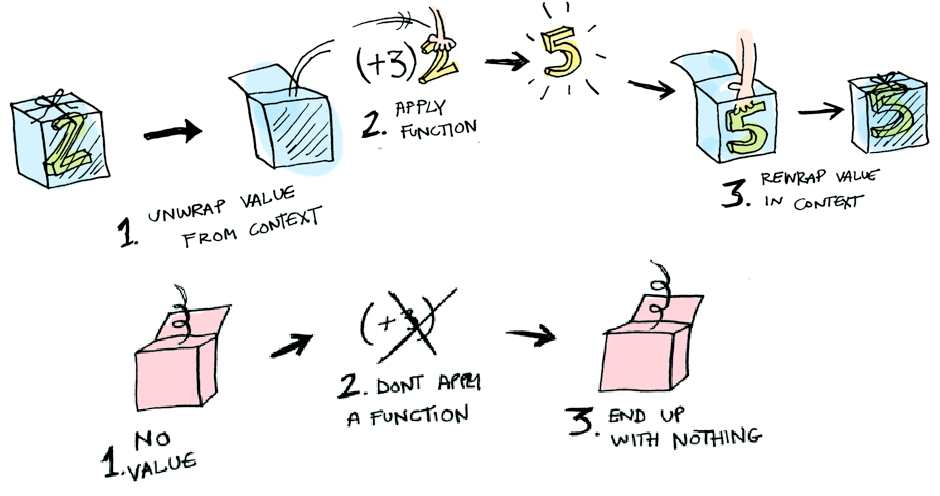
\includegraphics[scale=0.65]{images/functor}
\decoRule
\caption[functor]{Comportamento della funzione \textit{map} definita da Functor[Option] \cite{FunctorsApplicativesMonads}}
\end{figure}

Oltre a fornire la propria definizione del concetto di funtore, per i tipi per cui è implementato un funtore Scalaz abilita alcuni operatori iniettati che rendono disponibile il metodo \textit{map} e altri in grado di modificare la struttura dati di partenza come \textit{as}, \textit{fpair}, \textit{fproduct}, \textit{strengthL}, \textit{strengthR}, e \textit{void}.

Un aspetto molto interessante è costituito dal fatto che Scalaz definisce un'istanza di funtore anche per le funzioni, che in questo caso sono viste come una mappa infinita dal dominio al codominio. Così, usando il metodo \textit{map}, è possibile comporre due o più funzioni, anche se con un'anomalia non trascurabile: l'ordine è invertito rispetto alla classica composizione.

Tradizionalmente, la composizione di f e g porta ad ottenere una funzione corrispondente all'esecuzione di g seguita dall'esecuzione di f. Al contrario nei Functor di Scalaz, dato che \textit{map} è un metodo iniettato in F[A], la prima funzione eseguita è f e sul suo risultato viene poi applicata g.

\lstinputlisting[caption=Definizione di Functor e semplici esempi d'uso]{code/Functor.scala}

\subsection{Apply and Applicative}

Un funtore consente di applicare una funzione ad un valore all'interno di un contesto, ma se anche la funzione fosse racchiusa in un contesto? Per consentire l'applicazione della funzione nel caso descritto Scalaz introduce Apply[F[$\_$]], un'estensione di Functor[F] che espone un metodo \textit{ap}. Si tratta di una versione potenziata di \textit{map}, poiché estrae una funzione da un contesto e successivamente applica map su un valore usando la funzione estratta. 

Inoltre Scalaz abilita gli operatori iniettati <*>, alias simbolico per il metodo \textit{ap}, *> e <*, variazioni che restituiscono solo la parte destra o sinistra.

Scalaz raffina ulteriormente il concetto espresso con Apply, attraverso la definizione del trait Applicative[F[$\_$]]. Gli applicativi, oltre ad essere istanze di Apply, introducono il metodo \textit{point} (e il suo alias \textit{pure}) che prende un valore di qualsiasi tipo e lo restituisce all'interno del contesto per cui è stato definito l'applicativo. Inoltre, Scalaz inietta il metodo \textit{point} in tutti i tipi di dati consentendo così di trasformare un valore di tipo A in F[A].

\lstinputlisting[caption=Definizione di Apply e Applicative e esempi di utilizzo dell'operatore <*>]{code/Applicative.scala}

Seguendo lo stile introdotto con gli applicativi, Scalaz definisce anche una nuova notazione \textasciicircum(valore1, valore2, ...) \{ funzione \} che estrae i valori dai loro contesti e li applica ad una singola funzione (può essere utile perché consente di comportarsi come con gli applicativi senza dover inserire la funzione nel contesto). Questo nuovo stile presenta però un problema: non è in grado di gestire applicativi che accettano due parametri di tipo.

Per fornire lo stesso supporto anche a questi applicativi è stato introdotto \textit{Applicative Builder}, un'implementazione alternativa dello stile ispirato agli applicativi che usa la sintassi (valore1 |@| valore2 |@| ...) \{ funzione \}.

\lstinputlisting[caption=Esempi di \textit{Applicative Style} e \textit{Applicative Builder}]{code/ApplicativeStyle.scala}

\subsection{Monad}

Nei funtori il valore a cui viene applicata la funzione si trova in un contesto, negli applicativi anche la funzione stessa è all'interno del contesto e, infine, le monadi sono una naturale estensione degli applicativi nata per risolvere i casi in cui il valore è nel contesto e deve essere applicata una funzione che accetta un valore normale e ritorna un valore all'interno del contesto.

A differenza degli applicativi, le monadi dovranno essere in grado di estrarre il valore dal loro contesto per poi applicare la funzione data.

\begin{figure}[th]
\centering
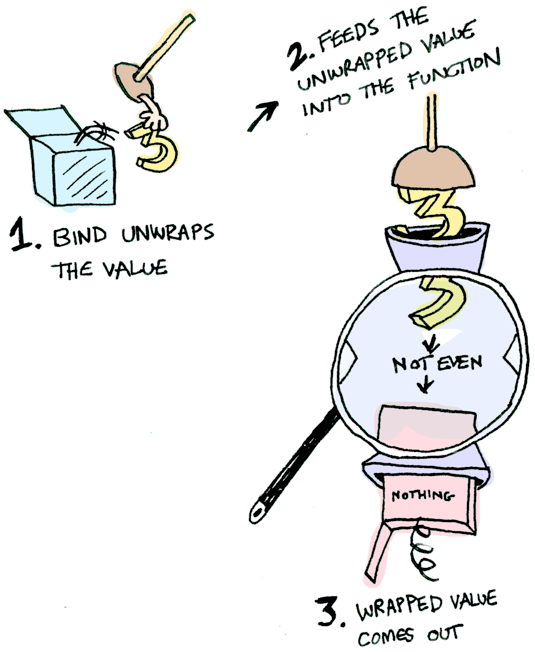
\includegraphics[scale=0.48]{images/monad}
\decoRule
\caption[monad]{Comportamento di una monade \cite{FunctorsApplicativesMonads}}
\end{figure}

Il trait Monad[F[\_]] mette a disposizione la definizione di monade di Scalaz, da cui si evince che tutte le monadi debbano essere istanze sia di Applicative[F] sia di Bind[F]. Quest'ultimo rappresenta ciò che le monadi hanno in più rispetto ai classici applicativi ed espone un metodo \textit{bind}, in grado di applicare una funzione A -> F[B] ad un valore nel suo contesto F[A]. Tutte le monadi dovranno inoltre rispettare le seguenti regole:

\begin{itemize}
\item \textit{Identità sinistra}: $\forall$ a, f, f(a) = bind(pure(a), f). Quindi se si prende un valore, si inserisce in un contesto con \textit{point} e si usa \textit{bind}, il risultato è lo stesso che si avrebbe applicando direttamente la funzione al valore.
\item \textit{Identità destra}: $\forall$ a, a = bind(a, x => pure (x)). L'elemento neutro della \textit{bind} è una funzione che restituisce il valore dato nel contesto.
\item \textit{Associatività}: $\forall$ a, f, g, bind(a, x => bind(f(x), g)) = bind(bind(a, f), g). Data una catena di applicazioni con funzioni monadiche, non importa come esse sono nidificate ma conta soltanto il loro ordine.
\end{itemize}

Come per gli altri costrutti visti, Scalaz fornisce ai tipi per cui è definita una monade il metodo \textit{bind} tramite l'operatore \textit{flatmap} e il suo alias >>=.

\lstinputlisting[caption=Definizione di Monad e dell'operatore \textit{flatMap}]{code/Monad.scala}

Un aspetto da tenere in grande considerazione quando si parla di monadi è il fatto che questo tipo di astrazioni, abilitando l'operatore \textit{flatMap}, possano essere usate in una \textit{for comprehension}. Così facendo, sarà possibile concatenare in modo semplice e leggibile una serie di applicazioni di funzione.

\lstinputlisting[caption=Semplice esempio di composizione monadica senza e con l'utilizzo della \textit{for comprehension}]{code/MonadFor.scala}

%----------------------------------------------------------------------------------------
%	SECTION 3
%----------------------------------------------------------------------------------------

\section{Type classes for error handling}

La programmazione funzionale prevede che il flusso di esecuzione del programma sia costituito da una serie di valutazioni matematiche, e il suo punto di forza è la mancanza di side effect. In caso di fallimento nell'esecuzione di una funzione (ad esempio, il mancato soddisfacimento di una condizione), è retaggio della programmazione imperativa l'utilizzo di eccezioni.

Il fatto che venga lanciata un'eccezione genera però un side effect, perché l'esecuzione del programma viene interrotta e continua in un luogo diverso rispetto a quello in cui si prevede che la funzione ritorni. Affinché sia completamente rispettato il paradigma funzionale, un linguaggio dovrebbe mettere a disposizione delle strutture dati in grado di incapsulare sia il valore atteso dalle funzioni sia un valore che rappresenta una condizione di errore.

Nella Scala Standard Library sono disponibili alcune astrazioni di questo tipo, che Scalaz va ad arricchire fornendo la propria implementazione dei costrutti già presenti e definendo delle nuove type class \cite{ScalazDummies}.

\subsection{Option}

La prima type class in grado di rappresentare un fallimento nell'applicazione di una funzione è Option[A], definita nella libreria standard e ampiamente usata, che offre la possibilità di ritornare o meno il risultato di una computazione. Scalaz fornisce un'estensione della sintassi disponibile per Option[A], aggiungendo metodi di costruzione alternativi e alcuni operatori unari.

In particolare, per i valori di qualsiasi tipo Scalaz fornisce il metodo \textit{some} con cui è possibile creare un option contenente quel valore. Il metodo none[A] consente invece di creare un option vuoto specificando già in fase di creazione di quale tipo sarà (per questo si differenzia da \textit{None.apply}).

\lstinputlisting[caption=Metodi introdotti per la costruzione di Option]{code/Option.scala}

Scalaz definisce inoltre alcuni operatori per le istanze di Option, tra cui:

\begin{itemize}
\item |, che costituisce un alias per il metodo \textit{getOrElse}.
\item $\sim$, ossia un alias per il metodo \textit{getOrElse} chiamato con argomento \textit{zero}.
\item ? a | b, statement che verifica se è presente un valore nell'Option, in tal caso restituisce a e in caso contrario b.
\end{itemize}

\subsection{Either \textbackslash/}

Mentre Option[A] consente di rappresentare l'assenza o la presenza di un errore, la type class Either[A, B] è in grado di inserire valori di successo in un contesto di possibile errore e di allegare un valore in caso di fallimento, in modo da poter fornire informazioni utili sull'errore che si è verificato.

Nella Scala Standard Library è definito Either[A, B], ma Scalaz fornisce la propria versione attraverso la definizione del trait \textbackslash/[A, B]. Per convenzione, la parte sinistra di \textbackslash/[A, B] viene usata per gli errori (il tipo A rappresenta un errore) e la parte destra è riservata agli esiti positivi. Le istanze di \textbackslash/[A, B] possono essere create con i metodi \textit{left} e \textit{right}, iniettati in tutti i tipi.

Scalaz accompagna la definizione di \textbackslash/[A, B] con metodi quali:

\begin{itemize}
\item \textit{isRight} e \textit{isLeft}, che controllano il lato da cui si trova il valore.
\item \textit{getOrElse} e il suo alias simbolico |, che restituiscono il valore nel lato destro o un valore di default in caso di errore.
\item \textit{swap} e il suo alias simbolico $\sim$, che invertono lato sinistro e destro.
\item \textit{map}, che è in grado di modificare il valore del lato destro.
\end{itemize}

Inizialmente \textbackslash/[A, B] era preferibile rispetto a Either[A, B], poiché l'implementazione di Scalaz è monadica ed espone il metodo \textit{flatMap}. Questo risulta essere molto comodo nella gestione degli errori, poiché abilita l'uso della \textit{for comprehension}. Tuttavia, nelle ultime versioni della libreria standard Either è diventata monadica ed ora la differenza è prettamente stilistica.

\lstinputlisting[caption=Combinazione di \textbackslash/ con una \textit{for comprehension}: fallimento in corrispondenza del primo valore sinistro]{code/Either.scala}

\subsection{Validation}

Either, o \textbackslash/ nella versione implementata da Scalaz, è uno strumento molto utile perché in grado di fornire una rappresentazione del fallimento. Pensiamo però ad uno scenario molto comune, in cui si verificano diversi errori nel corso della computazione e ognuno di essi è ritenuto importante.

Ad esempio, si consideri un form di registrazione in cui sono richiesti nome utente, password e conferma password. Affinché l'input dell'utente sia valido, il nome utente deve essere formato da un minimo di \textit{m} caratteri e non contenere caratteri speciali, la password deve essere composta da un minimo di \textit{n} caratteri e contenere almeno una lettera maiuscola e il campo di conferma deve essere uguale alla password. Nel caso in cui un utente commetta più errori, un buon sistema dovrebbe essere in grado di segnalarli tutti così che l'utente possa correggerli contemporaneamente.

Benché diversi valori di \textbackslash/ possano essere facilmente composti con una \textit{for comprehension}, la composizione assume un comportamento \textit{first-fail} poiché in caso di fallimento il valore restituito rappresenta solo il primo errore. Quindi \textbackslash/ non è adatto all'esempio: se l'utente commettesse un errore sia nel nome utente sia nella password, il secondo non sarebbe mostrato.

Partendo da questi presupposti, Scalaz introduce il trait Validation[E, A] e le sue implementazioni Success[E, A] e Failure[E, A]. Il costrutto Validation[E, A] è isomorfo a \textbackslash/[E, A] ed è infatti possibile convertirlo in esso tramite il metodo \textit{disjunction} (la conversione inversa è disponibile grazie al metodo \textit{validation}). Le istanze di Validation[E, A] possono essere create con i metodi \textit{success[E]} e \textit{failure[A]}, iniettati da Scalaz in tutti i tipi di dati.

A differenza di \textbackslash/[E, A], Validation[E, A] non è una monade ma, quando per E (il tipo che rappresenta l'errore in Validation[E, A]) è definito un semigruppo, esiste un Applicative[Validation[E, A]] in grado di accumulare gli errori. La sintassi più comune usata per unire le validazioni è quella proposta dall'\textit{Applicative Builder}, che consente di specificare solo la funzione con cui combinare i valori in caso di successo. Gli eventuali errori sono invece accumulati automaticamente secondo la politica stabilita dal semigruppo.

\lstinputlisting[caption=Creazione di Validation e loro composizione (possibile perché è definito un semigruppo per le stringhe)]{code/Validation.scala}

\subsection{ValidationNel}

Validation[E, A] consente di rappresentare nello stesso costrutto sia un possibile successo sia un insieme di fallimenti, ma se non fosse possibile combinare gli errori? O se si volesse mantenere la loro separazione? Ad esempio, dato un insieme di Validation[String, A], sarebbe possibile rappresentare gli errori come una concatenazione di stringhe, ma tutti i messaggi di errore sarebbero uniti in una stringa. Di certo, non si tratta della struttura dati ideale e sarebbe più naturale usare una collezione, come una semplice lista.

In questo contesto è utile il trait NonEmptyList[A], definito in Scalaz e a cui si fa riferimento con l'abbreviazione \textit{Nel}, che costituisce un wrapper per una lista, garantisce che essa non sia vuota e fa sì che il metodo \textit{head} sia sempre disponibile. Per la creazione delle istanze di NonEmptyList Scalaz mette a disposizione il metodo \textit{wrapNel}, iniettato in tutti i tipi di dati.

\lstinputlisting[caption=Definizione di NonEmptyList e costruzione usando il metodo \textit{wrapNel}]{code/NonEmptyList.scala}

Utilizzare \textit{Nel} e non una semplice lista come tipo per rappresentare gli errori in una validazione fa in modo che possa essere evitato, grazie al type system, il caso intrinsecamente ambiguo di \textit{Failure(List())}. Esso potrebbe infatti rappresentare infatti sia un fallimento sia l'assenza di errori.

Perciò Scalaz mette a disposizione ValidationNel[E, A], un type alias per Validation[NonEmptyList[E], A], \textit{successNel[E]} e \textit{failureNel[A]}, metodi iniettati in ogni tipo per la creazione di istanze di ValidationNel[E, A] \cite{ValidationNel}.

\lstinputlisting[caption=Esempi di creazione e composizione di ValidationNel]{code/ValidationNel.scala}

%----------------------------------------------------------------------------------------
%	SECTION 4
%----------------------------------------------------------------------------------------

\section{Useful features for everyday usage}

In aggiunta alle type class presentate nelle sezioni precedenti, Scalaz offre molti altri costrutti che possono essere un valido supporto per la programmazione. Di seguito saranno approfonditi alcuni di essi, ritenuti significativi e rivelatisi utili nell'implementazione del caso d'uso presentato.

\subsection{Tagging}

Il type system di Scala ha diverse potenzialità, come la possibilità di definire type alias in grado di rendere il codice più leggibile, ma non consente di limitare il range di supporto di un tipo. Si supponga ad esempio di voler esprimere una massa con il chilogrammo: si potrebbe usare un Double, ma come distinguerlo da altri Double che rappresentano concetti diversi?

La soluzione più semplice, e probabilmente la più naturale, consiste nel definire una case class \textit{KiloGram} contenente un solo parametro \textit{value} corrispondente alla massa (espressa attraverso un Double). In questo modo si ottiene la sicurezza dei tipi, ma si presentano i seguenti problemi:

\begin{itemize}
\item È necessario chiamare \textit{object.value} per estrarre il valore.
\item A runtime si verificheranno boxing e unboxing del valore, che comportano un maggiore costo di esecuzione. Sarà infatti allocato nello heap un oggetto wrapper (istanza della case class) contenente il valore, mentre sarebbe sufficiente mantenere quest'ultimo sullo stack.
\end{itemize}

Una soluzione alternativa è quella basata sui tipi taggati messi a disposizione da Scalaz \cite{TagTypes}. Il tagging consente di aggiungere ad un tipo dato un riferimento ad un altro tipo, andando così a definire un nuovo tipo. Inoltre, è stato introdotto l'alias di tipo @@ che, dati due tipi A e B, prevede che A with Tagged[B] possa essere rappresentato nella forma compatta A @@ B.

Scalaz fornisce il metodo \textit{Tag[A, B].apply}, con cui è possibile taggare un valore di tipo A con il tipo B. Per ottenere il valore presente nel tipo taggato è invece necessaria un'operazione di cast, disponibile grazie a \textit{Tag.unwrap}.

Facendo ancora riferimento alla rappresentazione del chilogrammo, sarà necessario definire un tipo \textit{KiloGram} (solitamente con un sealed trait) che sarà usato per taggare il tipo dei valori (Double). Double @@ KiloGram, che è un tipo vero e proprio e non un alias di tipo, sarà usato per rappresentare la massa. Qualora venga richiesto un valore di questo tipo, l'utente è obbligato a taggare il dato e in questo modo si ottiene la sicurezza dei tipi.

\lstinputlisting[caption=Definizione e esempio di tipo taggato (la funzione KiloGram tagga un valore di un qualsiasi tipo)]{code/Tag.scala}

Essendo necessario un cast esplicito per ottenere il valore presente all'interno del tipo taggato, in merito a questo aspetto non vi è un vantaggio concreto rispetto all'uso di case class (in cui è necessario chiamare \textit{object.value} per accedere al valore). Tuttavia, i tipi taggati portano i seguenti benefici:

\begin{itemize}
\item Non causano mai il boxing di un valore, perché il tipo taggato costituisce semplicemente il tipo che sarà associato al valore sullo stack.
\item Consentono di scrivere facilmente codice generico per i tipi taggati. Per esempio, Double @@ A rappresenta tutti i Double taggati con un qualche tipo ed è possibile definire una funzione generica per essi. Questo non sarebbe possibile se i Double fossero incapsulati in delle case class.
\end{itemize}

\subsection{Tree and TreeLoc}

Nella Scala Standard Library non è disponibile una struttura dati che consenta agli sviluppatori di rappresentare esplicitamente un albero. Benché sia semplice implementare un costrutto corrispondente a un albero, la realizzazione di algoritmi e procedure in grado di manipolarlo risulta essere decisamente complessa. Tra le varie strutture dati a complemento della libreria standard, Scalaz offre la propria implementazione di albero: Tree[A].

Tutte le istanze di Tree[A] sono dei multi-way tree, noti anche come rose tree, ossia strutture dati ad albero con un numero variabile e illimitato di rami per nodo. Ogni nodo dell'albero è a sua volta rappresentato come un albero (il sotto-albero radicato in quel nodo), contiene un elemento di tipo A (etichetta associata al nodo) e tutti gli alberi corrispondenti ai nodi figli.

Scalaz mette inoltre a disposizione i metodi \textit{leaf} e \textit{node}, iniettati in tutti i tipi di dati, che consentono di creare alberi. In particolare, il primo non accetta nessun argomento e crea un albero corrispondente ad una foglia (nodo senza figli) e il secondo costruisce un nodo avente come figli i nodi dati.

\lstinputlisting[caption={Definizione di Tree, delle sue modalità di costruzione e semplice esempio di utilizzo}]{code/Tree.scala}

Come già sottolineato, la complessità maggiore legata alla gestione dell'albero è costituita dalla realizzazione di strumenti in grado di manipolarlo. Tree[A] rappresenta un ottimo punto di partenza, ma come è possibile navigarlo? Come inserire un nodo nell'albero? Come verificare se un nodo è la radice dell'albero? Come accedere al nodo padre di un nodo dato?

Al momento Tree espone solo \textit{rootLabel} e \textit{subForest}, indubbiamente insufficienti per poter fare in modo semplice le operazioni appena elencate.

In quest'ambito si colloca il concetto di \textit{zipper}, un idioma che usa l'idea di ``contesto'' per manipolare le posizioni in una struttura dati. Uno zipper consente di prendere una struttura dati e concentrarsi su una sua parte, rendendo più semplici e più efficienti le operazioni di accesso e modifica.

Scalaz definisce TreeLoc[A], uno zipper per Tree[A] che rappresenta un albero e una posizione al suo interno. In particolare, nel TreeLoc sono mantenuti: il nodo attualmente selezionato, i fratelli a sinistra del nodo corrente, i fratelli a destra del nodo corrente e il contesto del suo nodo padre.

Nelle istanze di Tree[A] è disponibile il metodo \textit{loc}, che consente di generare il TreeLoc[A] corrispondente all'albero corrente. Ogni istanza di TreeLoc offre sia metodi capaci di spostare il focus all'interno dell'albero (e quindi di navigarlo) sia metodi in grado di aggiornare, inserire o eliminare degli elementi. Di seguito, sono riportate le funzionalità più significative:

\begin{itemize}
\item \textit{root}, che restituisce la radice dell'albero.
\item \textit{parent}, che ritorna il padre del nodo corrente.
\item \textit{left} e \textit{right}, che selezionano il fratello sinistro e destro del nodo corrente.
\item \textit{firstChild} e \textit{lastChild}, che restituiscono rispettivamente il figlio più a sinistra e quello più a destra del nodo corrente.
\item \textit{getChild}, che ritorna il figlio n-esimo del nodo corrente.
\item \textit{findChild}, che seleziona il primo figlio diretto del nodo corrente in grado di soddisfare il predicato dato.
\item \textit{modifyTree}, che modifica il nodo corrente con la funzione data.
\item \textit{modifyLabel}, che modifica l'etichetta del nodo corrente applicando la funzione specificata.
\item \textit{insertDownLast}, che inserisce il nodo figlio come ultimo figlio del nodo corrente e assegna a quest'ultimo il focus.
\end{itemize}

\lstinputlisting[caption=Definizione di TreeLoc]{code/TreeLoc.scala}

\subsection{State Monad}

Oltre ad esplicitare il concetto di monade fornendo un valido supporto a chiunque ne voglia definire una, Scalaz offre delle monadi standard pensate per operare in situazioni ricorrenti, tra cui è importante ricordare:

\begin{itemize}
\item \textbf{Reader Monad} Ogni azione è una funzione che ha come parametro l'ambiente. Un'azione può quindi leggere quanto contenuto nell'ambiente, ma non può modificare l'ambiente visto dalle azioni successive.
\item \textbf{Writer Monad} Ogni azione è una funzione che restituisce un valore da scrivere. Un'azione non può vedere quali altre azioni hanno già scritto, mentre i vari output accumulati sono disponibili al chiamante.
\item \textbf{State Monad} Ogni azione accetta un valore che rappresenta il vecchio stato e restituisce un valore dello stesso tipo corrispondente al nuovo stato. Un'azione può vedere lo stato in entrata e modificarlo prima di passarlo alla successiva. La state monad porta con sé un vincolo più stringente rispetto alle precedenti: dato che lo stato deve essere passato tra le varie computazioni, queste devono essere sequenziali.
\end{itemize}

Sia per motivi di tempo sia perché le monadi reader e writer non sono state usate nella realizzazione del caso d'uso presentato, saranno approfonditi soltanto funzionamento e implementazione della state monad \cite{ScalazStateMonad}.

A differenza del concetto generale di monade, StateMonad avvolge in modo specifico le funzioni. Si tratta di funzioni particolari, che accettano uno stato e restituiscono un valore insieme ad un nuovo stato, e rappresentano quindi una computazione con stato. In Scalaz, ogni state monad è istanza di State[S, A] ed è possibile utilizzare il companion object State per inizializzarne una partendo da una funzione nella forma \textit{s -> (a, s)}.

\lstinputlisting[caption=Creazione e composizione di StateMonad]{code/State.scala}

Nelll'esempio precedente l'oggetto State estende il trait StateFunctions, interessante perché contiene delle funzioni di supporto per operazioni che coinvolgono lo stato. Inoltre la \textit{for comprehension} riportata fa sì che venga generata una state monad in grado di eseguire in sequenza le tre computazioni, in cui lo stato condiviso è passato da ogni computazione alla successiva.

\lstinputlisting[caption=Funzioni di supporto definite in StateFunctions]{code/StateFunctions.scala}

Si consideri però il caso in cui una o più computazioni espresse tramite StateMonad possano fallire: è oneroso delegare la gestione degli errori alla logica interna della monade, la soluzione ideale sarebbe quella di includere la gestione dei fallimenti all'interno della state monad. Per poterlo fare è necessaria l'introduzione di un nuovo concetto, quello di \textit{monad transformer}. Si tratta di un'entità simile ad una monade che, a differenza di essa, non è autonoma ma modifica il comportamento di una monade sottostante.

Scalaz rappresenta il \textit{monad transformer} dedicato alla StateMonad con il trait StateT[F[\_], S, A]. Esso prevede che il risultato di ogni computazione sia incapsulato all'interno di un ``contenitore'' di tipo F e che da quest'ultimo dipendano le computazioni successive. Ad esempio, nel caso di State[Option, S, A] l'esecuzione di ogni computazione deve restituire Option[(S, A)] e, se dovesse verificarsi un fallimento, questo sarebbe propagato anche alle computazioni successive. In Scalaz State[S, A] è un ``banale'' type alias che fa riferimento a StateT[Id, S, A], dove Id corrisponde alla monade identità, poiché applica semplicemente la funzione incapsulata nella monade.

\lstinputlisting[caption=Definizione del \textit{monad transformer} StateT]{code/StateT.scala}
